\documentclass{beamer}

\usepackage[utf8]{inputenc}
\usepackage{hyperref}

\usetheme{Berkeley}
\beamertemplatenavigationsymbolsempty
\setbeamertemplate{headline}{}
 
\title{Erstellen eines Workflows in FoodChain-Lab 2}
\date{}
 
\begin{document}
\maketitle

\section{Aufgaben}
\begin{frame}
	\begin{itemize}
		\item Nutzen Sie den \textbf{Tracing View} um das Liefernetz in einer übersichtlichen Art und Weise darzustellen.
		\item Nutzen Sie das \textbf{Default Highlighting} zur farblichen Visualisierung.
		\item Visualisieren Sie den Forward- und Backward-Trace von einer beliebigen Station.
	\end{itemize}
\end{frame}
 
\section{1}
\begin{frame}
	\begin{center}
  		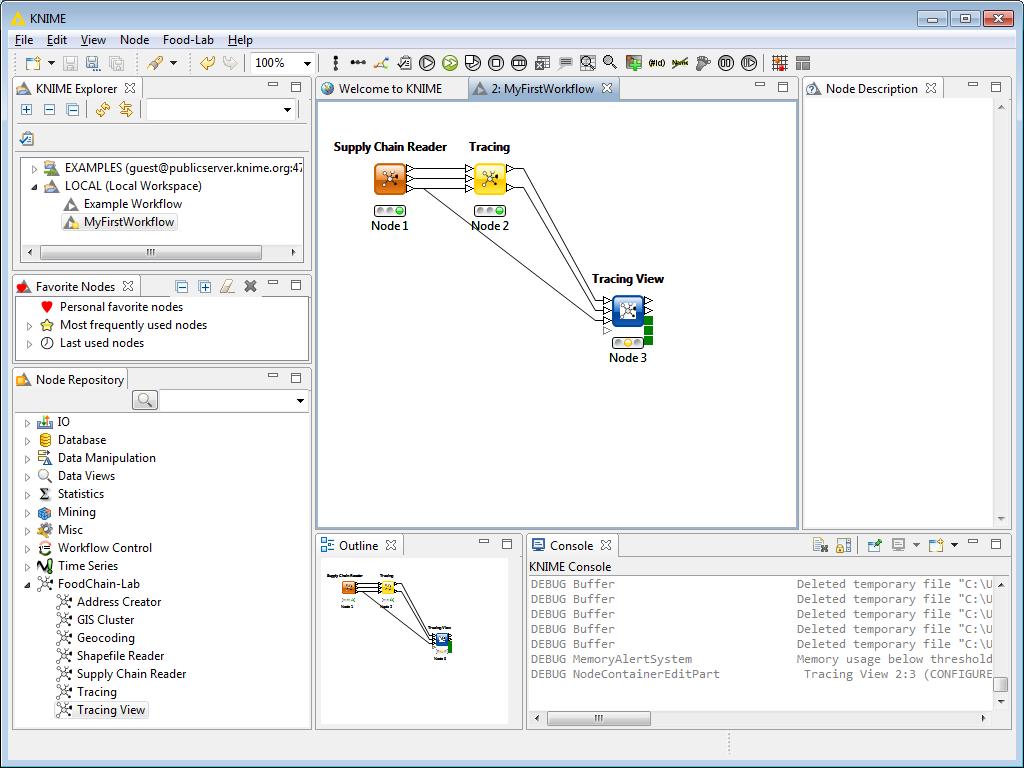
\includegraphics[height=0.5\textheight]{1.png}
	\end{center}
	\begin{itemize}
		\item Dies ist der zweite Teil des Tutorials.
		\item Sie können den Workflow aus Teil 1 entweder selber erstellen oder hier herunterladen: \url{https://github.com/SiLeBAT/BfROpenLabResources/raw/master/GitHubPages/workflows/My_First_Workflow.zip}.
		\item Machen Sie einen Doppelklick auf den \textbf{Tracing View} um den Dialog zu öffnen.
	\end{itemize}
\end{frame}

\section{2}
\begin{frame}
	\begin{center}
  		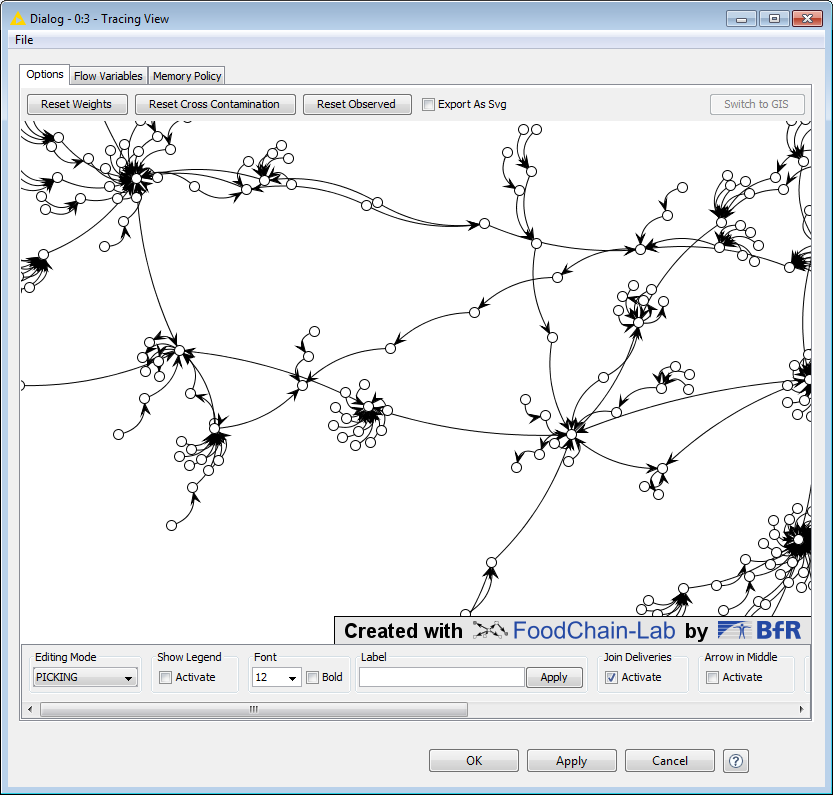
\includegraphics[height=0.6\textheight]{2.png}
	\end{center}
	\begin{itemize}
		\item Wenn Sie den \textbf{Tracing View} zum ersten Mal öffnen, werden Sie bemerken, dass sich die Stationen des Graphs bewegen. Dies liegt daran, dass der Layout-Prozess im Gange ist.
	\end{itemize}
\end{frame}

\section{3}
\begin{frame}
	\begin{center}
  		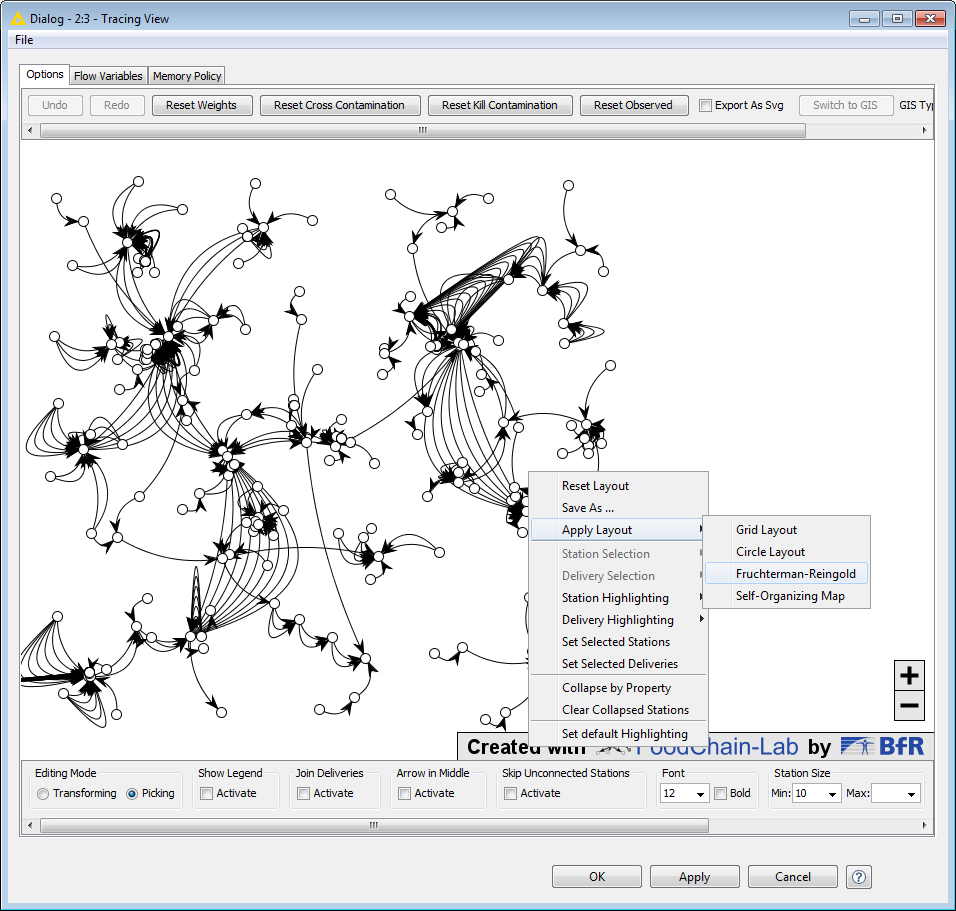
\includegraphics[height=0.6\textheight]{3.png}
	\end{center}
	\begin{itemize}
		\item Wenn der Layout-Prozess beendet ist, wählen Sie "TRANSFORMING" als \textbf{Editing Mode} and zoomen Sie bis Sie den ganzen Graph sehen können (Zoomen funktioniert wie in Google Maps).
	\end{itemize}
\end{frame}

\section{4}
\begin{frame}
	\begin{center}
  		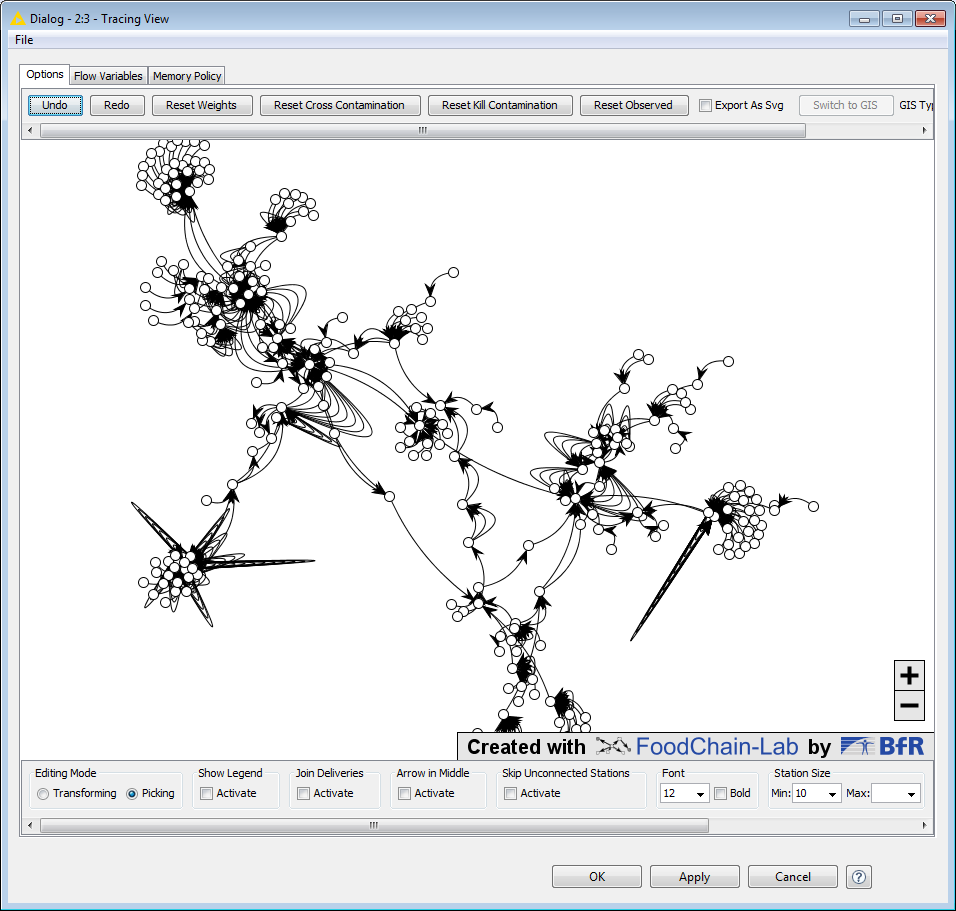
\includegraphics[height=0.6\textheight]{4.png}
	\end{center}
	\begin{itemize}
		\item Machen Sie einen Rechtsklick in den Graph um das Kontextmenü zu öffnen und wählen Sie \textbf{Set default Highlighting}.
		\item Beim Highlighting werden bestimmte Attribute von Stationen/Lieferungen mit Hilfe von Farben und Größen visualisiert.
	\end{itemize}
\end{frame}

\section{5}
\begin{frame}
	\begin{center}
  		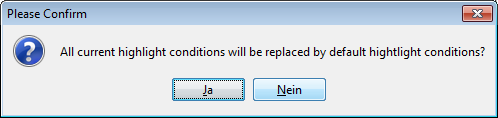
\includegraphics[width=0.9\textwidth]{5.png}
	\end{center}
	\begin{itemize}
		\item Im Dialog wählen Sie \textbf{Yes}.
	\end{itemize}
\end{frame}

\section{6}
\begin{frame}
	\begin{center}
  		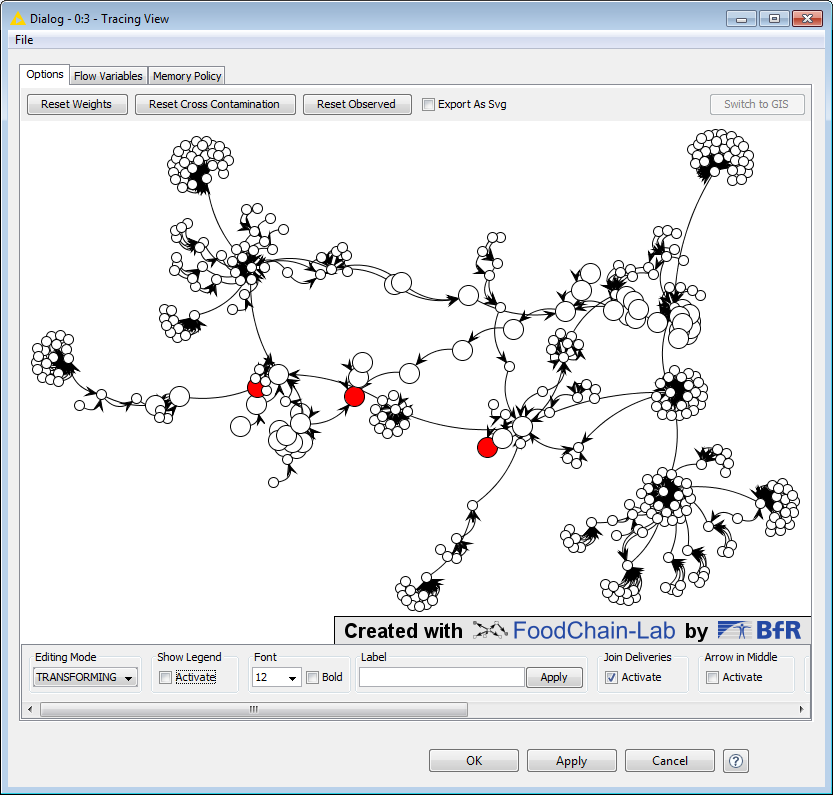
\includegraphics[height=0.6\textheight]{6.png}
	\end{center}
	\begin{itemize}
		\item Sie werden bemerken, dass drei Station nun rot gefärbt sind und manche Stationen größer sind als andere.
		\item Die roten Stationen sind die Supermärkte, bei denen wir das Gewicht auf "1" gesetzt haben.
		\item Die Größe jeder Station basiert nun auf ihrem "Score".
	\end{itemize}
\end{frame}

\section{7}
\begin{frame}
	\begin{center}
  		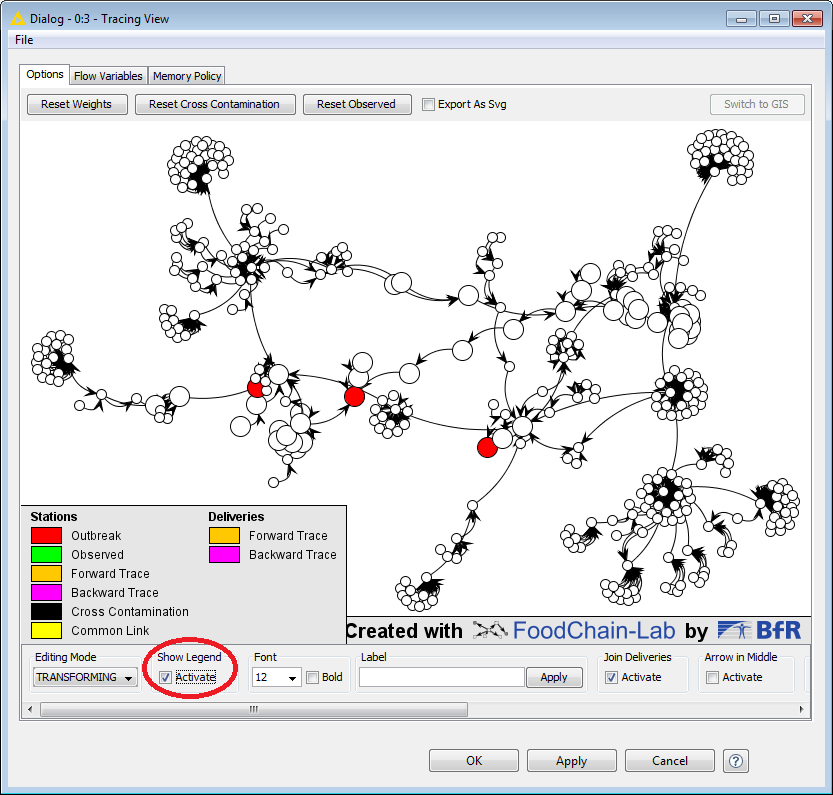
\includegraphics[height=0.6\textheight]{7.png}
	\end{center}
	\begin{itemize}
		\item Aktivieren Sie \textbf{Show Legend} um eine Legende für die benutzen Farben zu erhalten.
	\end{itemize}
\end{frame}

\section{8}
\begin{frame}
	\begin{center}
  		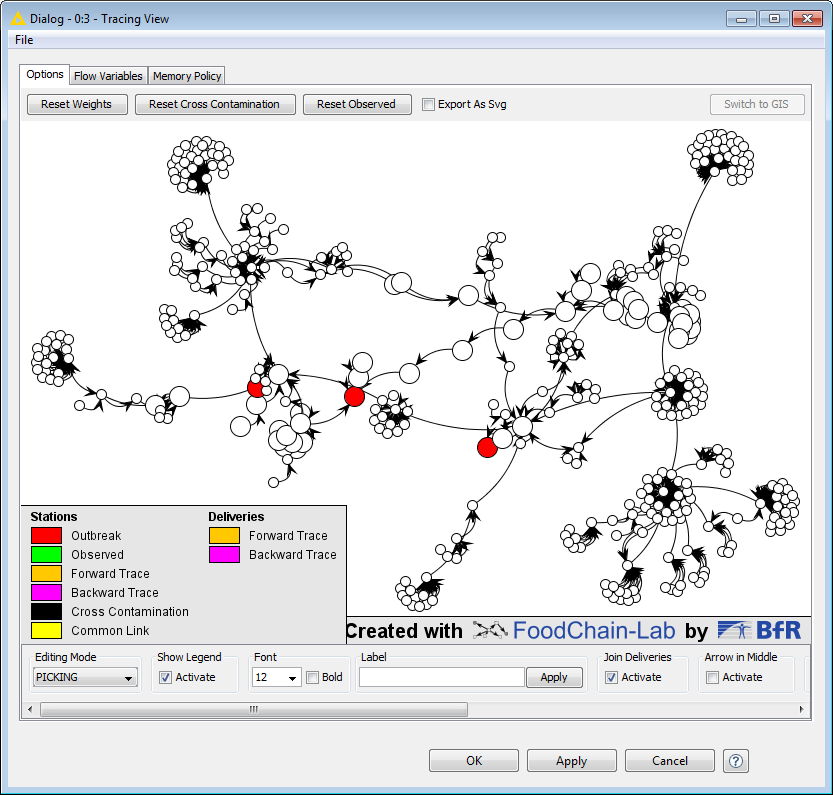
\includegraphics[height=0.6\textheight]{8.png}
	\end{center}
	\begin{itemize}
		\item Nun können wir eine Station als "Observed" markieren um uns ihren Trace anzeigen zu lassen.
		\item Setzen Sie "PICKING" als \textbf{Editing Mode} and machen Sie einen Doppelklick auf eine beliebige Station.
		\item Wir haben auf die Station im roten Kreis geklickt.
	\end{itemize}
\end{frame}

\section{9}
\begin{frame}
	\begin{center}
  		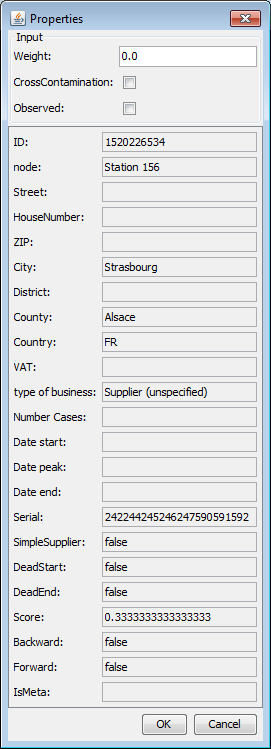
\includegraphics[height=0.6\textheight]{9.png}
	\end{center}
	\begin{itemize}
		\item Ein Dialog mit allen Attributen der gewählten Station erscheint.
		\item Oben im Dialog können Sie die Werte für "Weight", "Cross Contamination" und "Observed" verändern.		
	\end{itemize}
\end{frame}

\section{10}
\begin{frame}
	\begin{center}
  		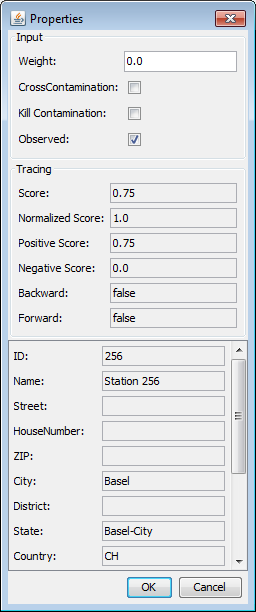
\includegraphics[height=0.6\textheight]{10.png}
	\end{center}
	\begin{itemize}
		\item Aktivieren Sie \textbf{Observed} und klicken Sie \textbf{OK}.
	\end{itemize}
\end{frame}

\section{11}
\begin{frame}
	\begin{center}
  		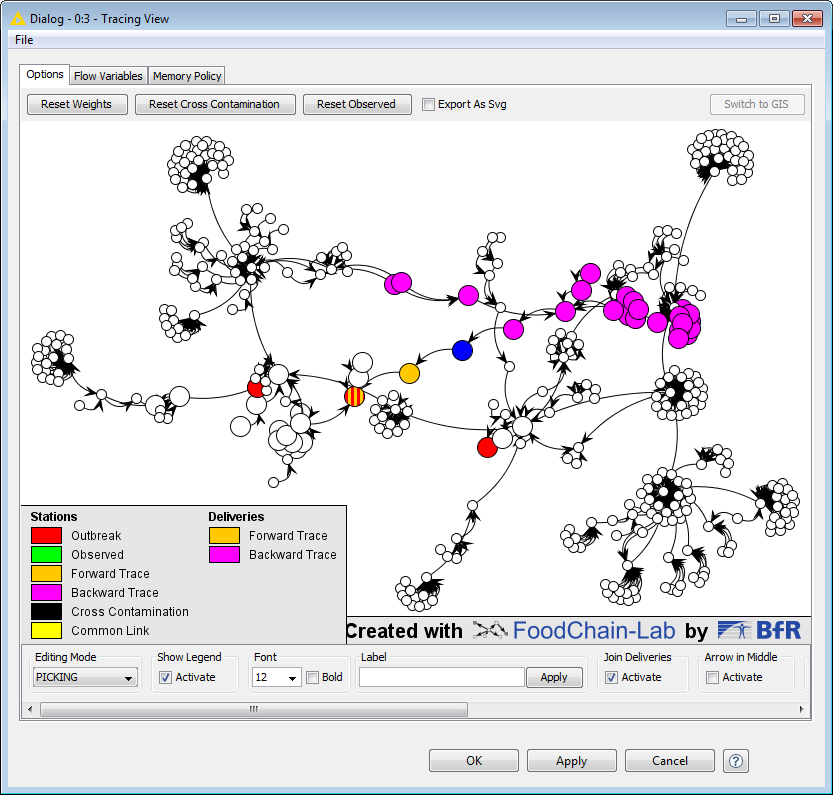
\includegraphics[height=0.6\textheight]{11.png}
	\end{center}
	\begin{itemize}
		\item Alle Stationen vom Forward-Trace sind orange gefärbt and die Stationen vom Backward-Trace sind magenta.
		\item Die Lieferungen werden nicht gefärbt solange die Option \textbf{Join Deliveries} aktiviert ist.
	\end{itemize}
\end{frame}

\section{12}
\begin{frame}
	\begin{center}
  		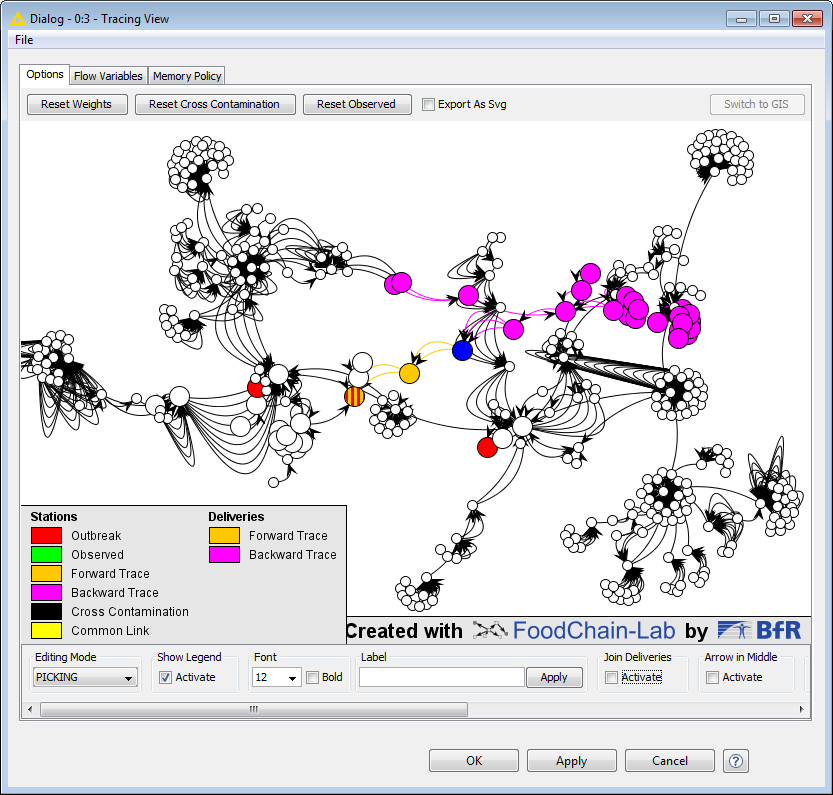
\includegraphics[height=0.6\textheight]{12.png}
	\end{center}
	\begin{itemize}
		\item Deaktivieren Sie \textbf{Join Deliveries}, damit jede Lieferung als einzelner Pfeil dargestellt wird.
		\item Nun sehen Sie, dass auch die Lieferungen vom Forward-/Backward-Trace gefärbt sind.
	\end{itemize}
\end{frame}

\end{document}